\section{Bilayer graphene}

In the tight-binding description of bilayer graphene, we take into account $2p_z$ orbitals on the four atomic sites in the unit cell, labelled as $j = A_1, B_1, A_2, B_2$. Then, the transfer integral matrix of bilayer graphene is a $4\times 4$  matrix given by \cite{McCann_2013}

\begin{equation}
    H(\vect k)=
    \begin{bmatrix}
        E_{A_1} & -\gamma_0 F(\vect k) & \gamma_4 F(\vect k) & -\gamma_3 F(\vect k)\\
        -\gamma_0 F(\vect k) & E_{B_1} & -\gamma_1 & \gamma_4 F(\vect k)\\
        \gamma_4 F(\vect k) & \gamma_1 & E_{A_2} & -\gamma_0 F(\vect k)\\
        -\gamma_3 F(\vect k)& \gamma_4 F(\vect k)& -\gamma_0 F(\vect k) & E_{B_2}
    \end{bmatrix}
\end{equation}

% 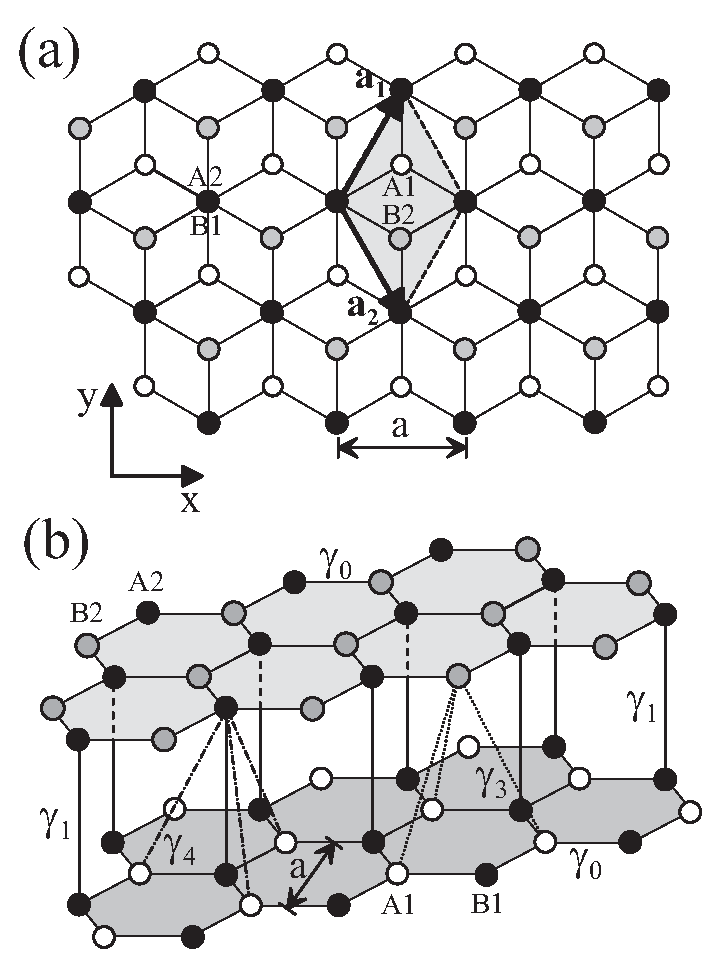
\includegraphics[width=\linewidth]{Immagini/graphene/bilayerlattice.eps}
% \caption{difference between the gapless and the gapped Dirac dispersion relation}
% \label{fig:bilayer-lattice}

\begin{table}[ht]
    \begin{minipage}[b]{0.56\linewidth}
    \centering
    \begin{tabular}{ l l r }
        \hline
        Parameter & Value [eV] \\ 
        \hline \hline
        $\gamma_0$ & $3.16\pm0.03$ \\
        $\gamma_1$ & $0.381\pm 0.003$ \\
        $\gamma_3$ & $0.38\pm 0.06$ \\
        $\gamma_4$ & $0.14\pm 0.03$ \\
        $s_0$ & boh\\
        $s_1$ & boh\\
        \hline
       \end{tabular}
        \caption{Values in eV of $\gamma_i$ \cite{kuzmenko2009determination}}
        \label{table:valuetable}
    \end{minipage}\hfill
    \begin{minipage}[b]{0.4\linewidth}
    \centering
    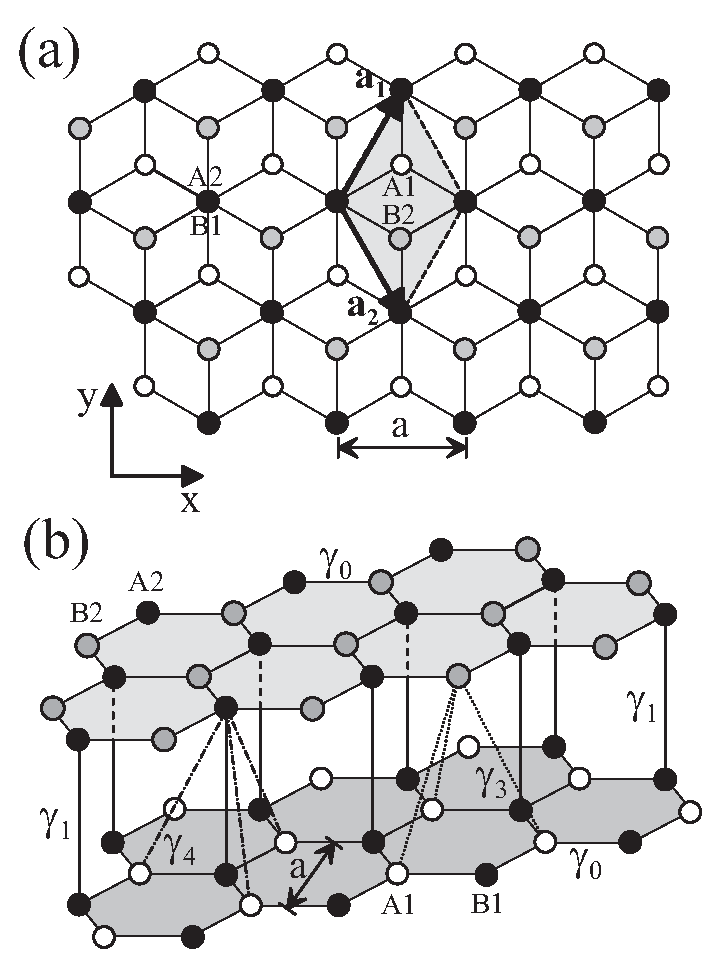
\includegraphics[width=\linewidth]{Immagini/graphene/bilayerlattice.eps}
    \captionof{figure}{Schematic representation of the bilayer graphene structure}
    \label{fig:bilayer-lattice}
    \end{minipage}
\end{table}

where the tight-binding parameters are defined as 
\begin{equation}
    \begin{split}
        \gamma_0=&-\braket{A_1|H}{B_1}=-\braket{A_2|H}{B_2} \\
        \gamma_1=&\braket{A_2|H}{B_1}  \\
        \gamma_3=&-\braket{A_1|H}{B_2}  \\
        \gamma_4=& \braket{A_1|H}{A_2}=\braket{B_1|H}{B_2} \\
    \end{split}
\end{equation}
The upper-right and lower-left square $2\times 2$ blocks of $H$ describe inter-layer coupling. Parameter $\gamma_1$ describes coupling between pairs of orbitals on sites that are directly above each other $B_1$ and $A_2$ (also called dimer sites): since this is a vertical coupling, the corresponding terms in $H$ do not contain $F(\vect k)$ which describes in-plane hopping. The other $\gamma$ factors do have an in plane component, which causes the $F(\vect k)$ term to show up.\\
The overlap matrix $S$ form equation $\ref{eq:overlap}$ becomes in the bilayer case
\begin{equation}
    S=
    \begin{bmatrix}
        1 & s_0 F(\vect k) & 0&0\\
        s_0 F(\vect k)  &1&s_1&0\\
        0&s_1&1&s_0 F(\vect k)\\
        0&0&s_0 F(\vect k) &1
    \end{bmatrix}
\end{equation}
Here we only include two parameters: $s_0 = \braket{A_1}{B_1} = \braket{A_2}{B_2}$ describing non-orthogonality of intra-layer nearest-neighbours and $s_1= \braket{A_2}{B_1}$ describing non-orthogonality of orbitals on dimer sites A1 and B2. In principle, it is possible to introduce additional parameters analogous to $\gamma_3,\gamma_4$, etc., but generally they will be small and irrelevant, infact in the bilayer case it is common practice to neglect completely the overlap matrix if we are dealing with. The resulting energy bands are plotted in figure \ref{fig:dispersion-bilayer}

\begin{figure}[h]
    \makebox[\textwidth][c]{
        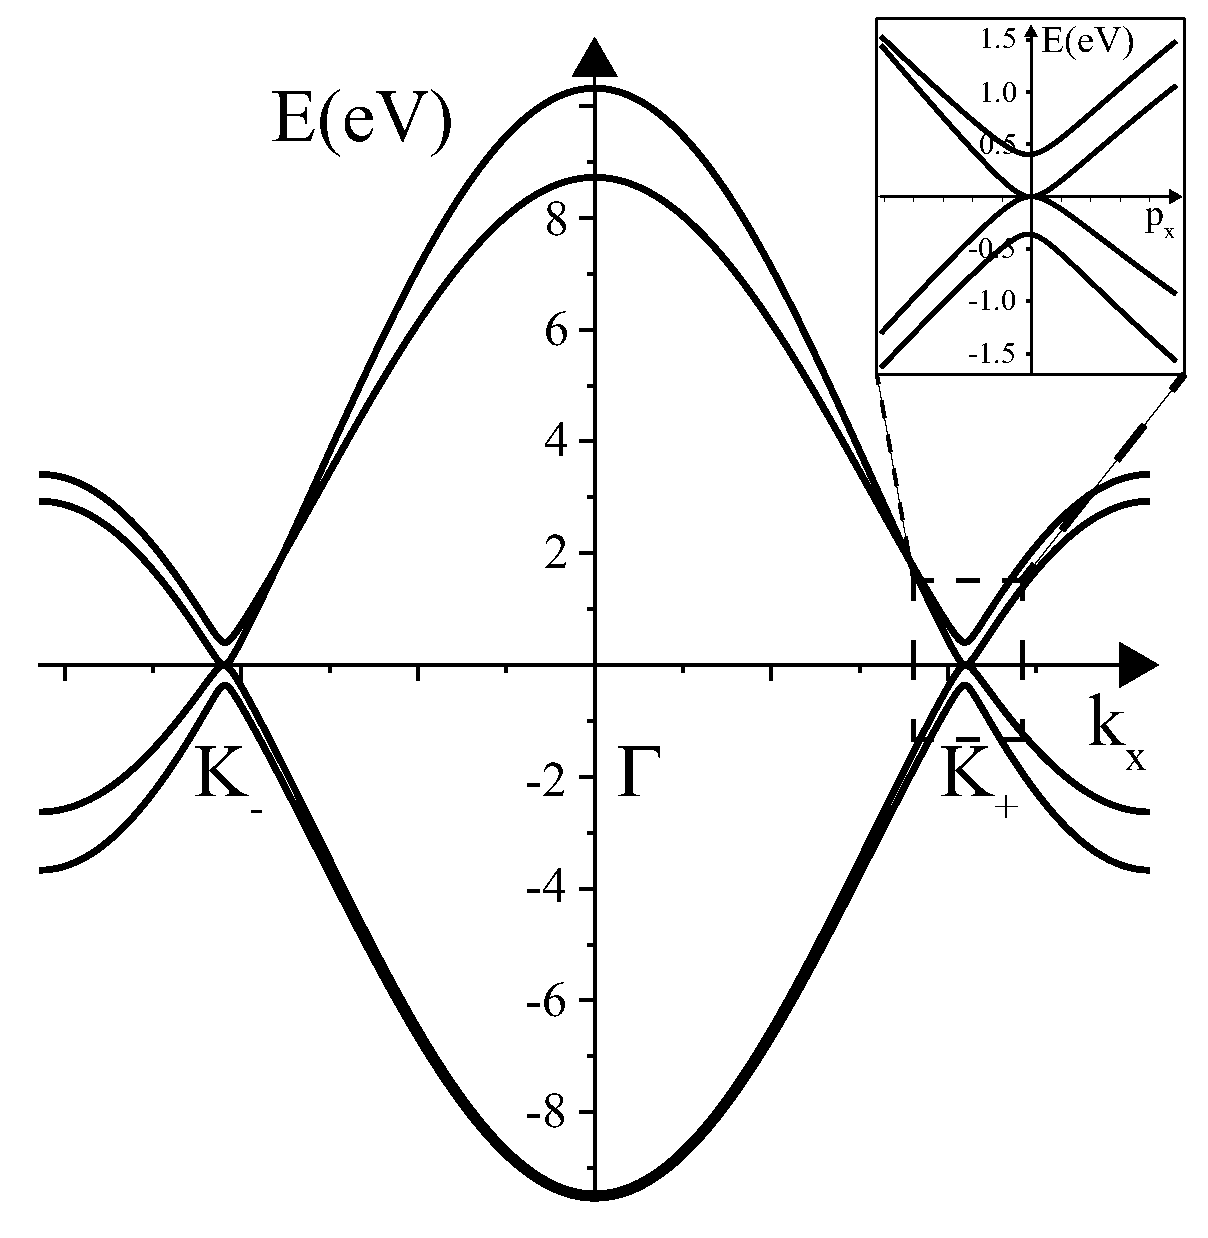
\includegraphics[width=.7\linewidth]{Immagini/graphene/bilayer-bands.eps}
        }%
    \caption{Here are plotted the $p_z$ orbitals along the $k_x$ axis in the reciprocal space intersecting the corners $K_0$ and $K_1$ and the center $\Gamma$ of the Brillouin zone. Notice how now we have four bands, this because we have four atoms in the fundamental cell, two for each layer}
    \label{fig:dispersion-bilayer}
\end{figure}
To describe the properties of the electrons near the $K$ we just have to approximate $F(\vect k)$ just like we did in equation \ref{eq:F(k)-approx}. This results in a Hamiltonian that is the generalization of the one we had in equation \ref{eq:gapped-dirac}

\begin{equation}
    H_{\vect K_0}=-H_{\vect K_1}^*=
    \begin{bmatrix}
        E_{A_1} & v_F\pi^\dag & -v_4\pi^\dag & v_3\pi\\
        v_F\pi& E_{B_1} & \gamma_1 & -v_4\pi^\dag\\
        -v_4\pi & \gamma_1 & E_{A_2} & v_F\pi^\dag\\
        v_3\pi^\dag & -v_4\pi & v_F\pi & E_{B_2}
    \end{bmatrix}
\end{equation}
Where $\pi= \hbar (k_x+ik_y),\pi^\dag=\hbar (k_x-ik_y)$, and the velocities $v_{3,4}=a\gamma_{3,4}/\hbar$ are effective fermi velocities that come from the coupling $\gamma_3$ and $\gamma_4$ CONTROLLA SE LA CONVERSIONE DELLA A è CORRETTA\\
A simple analytic solution may be obtained by neglecting the terms $v_4\pi$, $v_4\pi^\dag$ proportional to $\gamma_4$, and by considering only interlayer asymmetry $U$ in the on-site energies: $E_{A_1}=E_{B_1} = -U/2$ and $E_{A_2} = E_{B_2} = U/2$. Then, there is electron-hole symmetry, i.e., energies may be written $E = \pm E\alpha(\vect p), \alpha \in {1, 2}$

\begin{equation}
    \begin{split}
    &E_\alpha^2(\vect p)=\frac{ \gamma_1^2}2 + \frac{U^2}4+
    p^2\left(
        v^2+\frac{v^2_3}2
    \right)
    +(-1)^\alpha\,\sqrt{\Gamma}
    \\
    &\Gamma=\frac 14\left( \gamma_1^2-v_3^2p^2\right)^2+
    v^2p^2\left(\gamma_1^2+U^2+v_3^2p^2 \right)+ 
    2\zeta\gamma_1v_3v^2\cos(3\theta)
    \end{split}
\end{equation}
were $\theta$ is the polar angle of the impulse $\vect k=(k_x,k_y)=k(\cos\theta,\sin\theta)$
